\documentclass[../PS6_RapportFinal.tex]{subfiles}

\begin{document}
\graphicspath{{img/}{tex/img/}}
\subsection{Description de la réaction}

Afin de pouvoir soutirer un maximum d'énergie du tas de compost, il est nécessaire de connaître précisément la réaction chimique du compostage d'une matière organique.La connaissance des facteurs influents nous permettra d'y apporter une attention particulière et ainsi améliorer l'efficacité de la réaction.

\subsubsection{Dégradation anaérobie}
En absence de dioxygène, la biodégradation du compost se déroule suivant 4 phases :
\begin{itemize}
\item La phase d’hydrolyse : les composants de la matière organique sont décomposés en leurs molécules constitutives élémentaires par les enzymes (notés \(\mu\)). C’est une phase de préparation.

\item La phase acidogène : les sucres et acides aminés vont se dégrader pour produire de l'acide (essentiellement de l'acétate).
%eqn
\[C_6H_{12}O_5 +2H_2O \longrightarrow 2 CH_3COOH + 2CO_2 + 4 H_2\]
	


\item La phase acétogenèse : les acides et alcools formés lors des 2 précédentes phases sont transformés en acétate, dioxyde de carbone et dihydrogène.

\item La phase méthanogène : c’est lors de cette phase que vont être émis la plupart des gaz à effet de serre  
%eqn
\[CH_3COOH \longrightarrow CH_4 + H_2\]
\[4H_2 + CO_2 \longrightarrow  CH_4 + CO_2\]

\end{itemize}

\vspace{3mm}

La biodégradation de Matière Organique (MO ou \(C_aH_bO_c\)) réelle obéit à l’équation chimique suivante :
%eqn
\[MO + H_2O \stackrel{\mu}{\longrightarrow} n_\mu + MO_{recalcitrante} +CO_2 + CH_4 + gaz divers\]

Si l’on considère la réaction comme \og totale\fg{} on obtient :
%eqn
\[C_aH_bO_c + \frac{4a - b - 2c -3d}{4}H_2O \longrightarrow \frac{4a + b - 2c}{8}CH_4+ \frac{4a-b+2c}{8} CO_2\]

On observe que cette réaction dégage du méthane qui est 4 fois plus polluant que le \(CO_{2}\). Il faudrait donc limiter le dégagement de méthane. Cependant, il existe une autre réaction de décomposition possible.

\subsubsection{Dégradation aérobie}
En présence de dioxygène, la dégradation du compost s'organise selon 3 phases :
\begin{itemize}
\item La phase mésophile : la matière organique c'est-à-dire les substrats et la matière biodégradable sont métabolisés (transformation d’un substrat par des enzymes) par les bactéries mésophiles (moyennes températures). Cette phase dure de 5 à 10 jours et il peut y avoir une augmentation de température dans le compost de l’ordre de 30\degres C en 24h.

\item La phase thermophile : dans cette phase il y a une prédominance des bactéries thermophiles. La température dans le compost monte jusqu'à 70\degres C à cause de l’activité microbienne.

\item La phase de maturation : le reste de la matière organique est détruite pour devenir de la matière carbonée (minéralisation). On voit aussi la création d’acide fulvique et humique.
\end{itemize}
\vspace{3mm}

\begin{figure}[!h]
\begin{center}
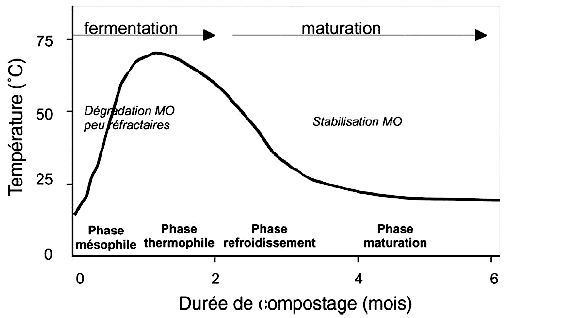
\includegraphics[width=15cm]{1_1_2_evolutiontemperature.png}
\caption{Évolution de la température dans le tas de compost}
\end{center}
\end{figure}

La biodégradation de matière organique réelle obéit à l’équation chimique suivante :
%eqn
\[MO + O_2 + sels \stackrel{\mu}{\longrightarrow} n_\mu + MO_{recalcitrante} +CO_2 +H_2O + chaleur\]

Si l’on considère la réaction comme "totale" on obtient :
%eqn
\[C_aH_bO_cN_d + \frac{4a + b - 2c -3d}{4}O_2 \longrightarrow aCO_2+ \frac{b-3d}{2} H_2O + dNH_3\]

Cette réaction est bien meilleure d'un point de vue écologique; en effet on ne rejette plus de méthane mais uniquement du \(CO_{2}\) qui est 4 fois moins polluant. Cependant, il faut que le dioxygène soit présent en quantité suffisante dans le tas de compost. De plus on observe l'apparition d'ammoniac (\(NH_{3}\)). Néanmoins dans notre cas, la matière organique (\(C_aH_bO_cN_d\)) ne contient pas d'azote donc on aura pas d'ammoniac dans notre tas de compost.
\end{document}